%% ---------------------------------------------------
%% Notice that we use the "report" class instead of "article"
%% ---------------------------------------------------
\documentclass{report}

\title{Blue Beer\\
 Expansion Project\\
  Picasso\\
 \textbf{Codebook}}
\author{Karl Jurek\\
Travis Daun\\
Joe Jiang}
\date{\today}

%% ---------------------------------------------------
%% 634format specifies the format of our reports
%% ---------------------------------------------------
\usepackage{634format}

%% ---------------------------------------------------
%% enumerate 
%% ---------------------------------------------------
\usepackage{enumerate}

%% ---------------------------------------------------
%% listings is used for including our source code in reports
%% textcomp provides additional symbols
%% ---------------------------------------------------
\usepackage{listings}
\usepackage{textcomp}
\usepackage{pdfpages}

%% ---------------------------------------------------
%% Packages for math environments
%% ---------------------------------------------------
\usepackage{amsmath}

%% ---------------------------------------------------
%% Packages for URLs and hotlinks in the table of contents
%% and symbolic cross references using \ref
%% ---------------------------------------------------
\usepackage{hyperref}

\usepackage[most]{tcolorbox}
\usepackage[utf8]{inputenc}
\usepackage{color,soul}
\usepackage{pgfplots}

%% ---------------------------------------------------
%% Packages for using HOL-generated macros and displays
%% ---------------------------------------------------
\usepackage{holtex}
\usepackage{holtexbasic}
% =====================================================================
%
% Macros for typesetting the HOL system manual
%
% =====================================================================

% ---------------------------------------------------------------------
% Abbreviations for words and phrases
% ---------------------------------------------------------------------

\newcommand\TUTORIAL{{\footnotesize\sl TUTORIAL}}
\newcommand\DESCRIPTION{{\footnotesize\sl DESCRIPTION}}
\newcommand\REFERENCE{{\footnotesize\sl REFERENCE}}
\newcommand\LOGIC{{\footnotesize\sl LOGIC}}
\newcommand\LIBRARIES{{\footnotesize\sl LIBRARIES}}
\usepackage{textcomp}

\newcommand{\bs}{\texttt{\char'134}} % backslash
\newcommand{\lb}{\texttt{\char'173}} % left brace
\newcommand{\rb}{\texttt{\char'175}} % right brace
\newcommand{\td}{\texttt{\char'176}} % tilde
\newcommand{\lt}{\texttt{\char'74}} % less than
\newcommand{\gt}{\texttt{\char'76}} % greater than
\newcommand{\dol}{\texttt{\char'44}} % dollar
\newcommand{\pipe}{\texttt{\char'174}}
\newcommand{\apost}{\texttt{\textquotesingle}}
% double back quotes ``
\newcommand{\dq}{\texttt{\char'140\char'140}}
%These macros were included by slind:

\newcommand{\holquote}[1]{\dq#1\dq}

\def\HOL{\textsc{Hol}}
\def\holn{\HOL}  % i.e. hol n(inety-eight), no digits in
                 % macro names is a bit of a pain; deciding to do away
                 % with hol98 nomenclature means that we just want to
                 % write HOL for hol98.
\def\holnversion{Kananaskis-11}
\def\holnsversion{Kananaskis~11} % version with space rather than hyphen
\def\LCF{{\small LCF}}
\def\LCFLSM{{\small LCF{\kern-.2em}{\normalsize\_}{\kern0.1em}LSM}}
\def\PPL{{\small PP}{\kern-.095em}$\lambda$}
\def\PPLAMBDA{{\small PPLAMBDA}}
\def\ML{{\small ML}}
\def\holmake{\texttt{Holmake}}

\newcommand\ie{\mbox{\textit{i{.}e{.}}}}
\newcommand\eg{\mbox{\textit{e{.}g{.}}}}
\newcommand\viz{\mbox{viz{.}}}
\newcommand\adhoc{\mbox{\it ad hoc}}
\newcommand\etal{{\it et al.\/}}
% NOTE: \etc produces wrong spacing if used between sentences, that is
% like here \etc End such sentences with non-macro etc.
\newcommand\etc{\mbox{\textit{etc{.}}}}

% ---------------------------------------------------------------------
% Simple abbreviations and macros for mathematical typesetting
% ---------------------------------------------------------------------

\newcommand\fun{{\to}}
\newcommand\prd{{\times}}

\newcommand\conj{\ \wedge\ }
\newcommand\disj{\ \vee\ }
\newcommand\imp{ \Rightarrow }
\newcommand\eqv{\ \equiv\ }
\newcommand\cond{\rightarrow}
\newcommand\vbar{\mid}
\newcommand\turn{\ \vdash\ } % FIXME: "\ " results in extra space
\newcommand\hilbert{\varepsilon}
\newcommand\eqdef{\ \equiv\ }

\newcommand\natnums{\mbox{${\sf N}\!\!\!\!{\sf N}$}}
\newcommand\bools{\mbox{${\sf T}\!\!\!\!{\sf T}$}}

\newcommand\p{$\prime$}
\newcommand\f{$\forall$\ }
\newcommand\e{$\exists$\ }

\newcommand\orr{$\vee$\ }
\newcommand\negg{$\neg$\ }

\newcommand\arrr{$\rightarrow$}
\newcommand\hex{$\sharp $}

\newcommand{\uquant}[1]{\forall #1.\ }
\newcommand{\equant}[1]{\exists #1.\ }
\newcommand{\hquant}[1]{\hilbert #1.\ }
\newcommand{\iquant}[1]{\exists ! #1.\ }
\newcommand{\lquant}[1]{\lambda #1.\ }

\newcommand{\leave}[1]{\\[#1]\noindent}
\newcommand\entails{\mbox{\rule{.3mm}{4mm}\rule[2mm]{.2in}{.3mm}}}

% ---------------------------------------------------------------------
% Font-changing commands
% ---------------------------------------------------------------------

\newcommand{\theory}[1]{\hbox{{\small\tt #1}}}
\newcommand{\theoryimp}[1]{\texttt{#1}}

\newcommand{\con}[1]{{\sf #1}}
\newcommand{\rul}[1]{{\tt #1}}
\newcommand{\ty}[1]{\textsl{#1}}

\newcommand{\ml}[1]{\mbox{{\def\_{\char'137}\texttt{#1}}}}
\newcommand{\holtxt}[1]{\ml{#1}}
\newcommand\ms{\tt}
\newcommand{\s}[1]{{\small #1}}

\newcommand{\pin}[1]{{\bf #1}}
% FIXME: for multichar symbols \mathit should be used.
\def\m#1{\mbox{\normalsize$#1$}}

% ---------------------------------------------------------------------
% Abbreviations for particular mathematical constants etc.
% ---------------------------------------------------------------------

\newcommand\T{\con{T}}
\newcommand\F{\con{F}}
\newcommand\OneOne{\con{One\_One}}
\newcommand\OntoSubset{\con{Onto\_Subset}}
\newcommand\Onto{\con{Onto}}
\newcommand\TyDef{\con{Type\_Definition}}
\newcommand\Inv{\con{Inv}}
\newcommand\com{\con{o}}
\newcommand\Id{\con{I}}
\newcommand\MkPair{\con{Mk\_Pair}}
\newcommand\IsPair{\con{Is\_Pair}}
\newcommand\Fst{\con{Fst}}
\newcommand\Snd{\con{Snd}}
\newcommand\Suc{\con{Suc}}
\newcommand\Nil{\con{Nil}}
\newcommand\Cons{\con{Cons}}
\newcommand\Hd{\con{Hd}}
\newcommand\Tl{\con{Tl}}
\newcommand\Null{\con{Null}}
\newcommand\ListPrimRec{\con{List\_Prim\_Rec}}


\newcommand\SimpRec{\con{Simp\_Rec}}
\newcommand\SimpRecRel{\con{Simp\_Rec\_Rel}}
\newcommand\SimpRecFun{\con{Simp\_Rec\_Fun}}
\newcommand\PrimRec{\con{Prim\_Rec}}
\newcommand\PrimRecRel{\con{Prim\_Rec\_Rel}}
\newcommand\PrimRecFun{\con{Prim\_Rec\_Fun}}

\newcommand\bool{\ty{bool}}
\newcommand\num{\ty{num}}
\newcommand\ind{\ty{ind}}
\newcommand\lst{\ty{list}}

% ---------------------------------------------------------------------
% \minipagewidth = \textwidth minus 1.02 em
% ---------------------------------------------------------------------

\newlength{\minipagewidth}
\setlength{\minipagewidth}{\textwidth}
\addtolength{\minipagewidth}{-1.02em}

% ---------------------------------------------------------------------
% Environment for the items on the title page of a case study
% ---------------------------------------------------------------------

\newenvironment{inset}[1]{\noindent{\large\bf #1}\begin{list}%
{}{\setlength{\leftmargin}{\parindent}%
\setlength{\topsep}{-.1in}}\item }{\end{list}\vskip .4in}

% ---------------------------------------------------------------------
% Macros for little HOL sessions displayed in boxes.
%
% Usage: (1) \setcounter{sessioncount}{1} resets the session counter
%
%        (2) \begin{session}\begin{verbatim}
%             .
%              < lines from hol session >
%             .
%            \end{verbatim}\end{session}
%
%            typesets the session in a numbered box.
% ---------------------------------------------------------------------

\newlength{\hsbw}
\setlength{\hsbw}{\textwidth}
\addtolength{\hsbw}{-\arrayrulewidth}
\addtolength{\hsbw}{-\tabcolsep}
\newcommand\HOLSpacing{13pt}

\newcounter{sessioncount}
\setcounter{sessioncount}{0}

\newenvironment{session}{\begin{flushleft}
 \refstepcounter{sessioncount}
 \begin{tabular}{@{}|c@{}|@{}}\hline
 \begin{minipage}[b]{\hsbw}
 \vspace*{-.5pt}
 \begin{flushright}
 \rule{0.01in}{.15in}\rule{0.3in}{0.01in}\hspace{-0.35in}
 \raisebox{0.04in}{\makebox[0.3in][c]{\footnotesize\sl \thesessioncount}}
 \end{flushright}
 \vspace*{-.55in}
 \begingroup\small\baselineskip\HOLSpacing}{\endgroup\end{minipage}\\ \hline
 \end{tabular}
 \end{flushleft}}

% ---------------------------------------------------------------------
% Macro for boxed ML functions, etc.
%
% Usage: (1) \begin{holboxed}\begin{verbatim}
%               .
%               < lines giving names and types of mk functions >
%               .
%            \end{verbatim}\end{holboxed}
%
%            typesets the given lines in a box.
%
%            Conventions: lines are left-aligned under the "g" of begin,
%            and used to highlight primary reference for the ml function(s)
%            that appear in the box.
% ---------------------------------------------------------------------

\newenvironment{holboxed}{\begin{flushleft}
  \begin{tabular}{@{}|c@{}|@{}}\hline
  \begin{minipage}[b]{\hsbw}
% \vspace*{-.55in}
  \vspace*{.06in}
  \begingroup\small\baselineskip\HOLSpacing}{\endgroup\end{minipage}\\ \hline
  \end{tabular}
  \end{flushleft}}

% ---------------------------------------------------------------------
% Macro for unboxed ML functions, etc.
%
% Usage: (1) \begin{hol}\begin{verbatim}
%               .
%               < lines giving names and types of mk functions >
%               .
%            \end{verbatim}\end{hol}
%
%            typesets the given lines exactly like {boxed}, except there's
%            no box.
%
%            Conventions: lines are left-aligned under the "g" of begin,
%            and used to display ML code in verbatim, left aligned.
% ---------------------------------------------------------------------

\newenvironment{hol}{\begin{flushleft}
 \begin{tabular}{c@{}@{}}
 \begin{minipage}[b]{\hsbw}
% \vspace*{-.55in}
 \vspace*{.06in}
 \begingroup\small\baselineskip\HOLSpacing}{\endgroup\end{minipage}\\
 \end{tabular}
 \end{flushleft}}

% ---------------------------------------------------------------------
% Emphatic brackets
% ---------------------------------------------------------------------

\newcommand\leb{\lbrack\!\lbrack}
\newcommand\reb{\rbrack\!\rbrack}


% ---------------------------------------------------------------------
% Quotations
% ---------------------------------------------------------------------


%These macros were included by ap; they are used in Chapters 9 and 10
%of the HOL DESCRIPTION

\newcommand{\inds}%standard infinite set
 {\mbox{\rm I}}

\newcommand{\ch}%standard choice function
 {\mbox{\rm ch}}

\newcommand{\den}[1]%denotational brackets
 {[\![#1]\!]}

\newcommand{\two}%standard 2-element set
 {\mbox{\rm 2}}

\pgfmathdeclarefunction{gauss}{3}{%
  \pgfmathparse{1/(#3*sqrt(2*pi))*exp(-((#1-#2)^2)/(2*#3^2))}%
}
\begin{document}

%% --------------------------------------------------- the listings
%% parameter "language" is set to "ML"
%% ---------------------------------------------------
\lstset{language=R,
    basicstyle=\small\ttfamily,
    stringstyle=\color{DarkGreen},
    otherkeywords={0,1,2,3,4,5,6,7,8,9},
    morekeywords={TRUE,FALSE},
    deletekeywords={data,frame,length,as,character},
    keywordstyle=\color{blue},
    commentstyle=\color{DarkGreen},
}
\lstset{language=SAS, 
  breaklines=true,  
  basicstyle=\ttfamily\bfseries,
  columns=fixed,
  keepspaces=true,
  identifierstyle=\color{blue}\ttfamily,
  keywordstyle=\color{cyan}\ttfamily,
  stringstyle=\color{purple}\ttfamily,
  commentstyle=\color{green}\ttfamily,
  } 

\maketitle{}

\tableofcontents{}

%% -----------------------------------------------------------
%% Warning: don't copy and paste chapter, section, and subsection
%% commands with their labels.  This degrades/confuses cross
%% references and URL hotlinks within your document!
%% Use C-c C-s to introduce new sections and labels.
%% If automatic labels don't work right, execute M-x reftex-mode
%% (usually twice) to toggle reftex (automatic labeling) off and
%% on.
%% -----------------------------------------------------------

\chapter{Executive Summary}
\label{cha:executive-summary}

We wish to develop a strategy for the deployment of a new beer, Blue Beer's Picasso.
Blue Beer's Picasso has higher than typical alcohol content (ABV= 0.06) while having
a lower than typical bitterness rating (IBU = 30). Market research has shown that Millennials and iGen ($>=21$) prefer locally brewed beers, that have a high alcohol content but are not drawn to highly bitter beers. Blue Beer's Picasso is looking to launch their brewery production in an area with fewer than 10 breweries in the state, has a supporting demographic, and prefers beers  with Blue Beer's ABV and IBU characteristics.\\

\noindent The data analysis performed can be found in \emph{JKT_Final.Rmd}. This codebook will provide information on the datasets used, the methods employed, and the pertinent information on how results were obtained to aid in the reproduction of our results. 
\begin{center}

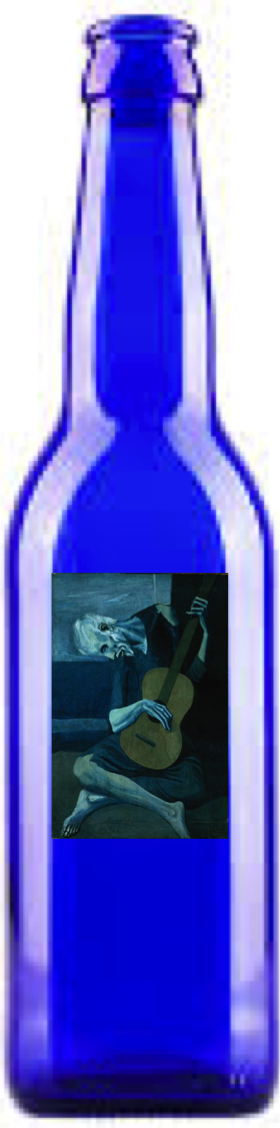
\includegraphics[scale=.5]{../graphics/beer2}

\end{center}

\chapter{R and RStudio}
\label{cha:RStudio}

\section{Version}
\label{sec:RVersion}
\begin{verbatim}
R version 3.5.1 (2018-07-02)
Platform: x86_64-apple-darwin15.6.0 (64-bit)
Running under: macOS Sierra 10.12.6
\end{verbatim}

\section{Base Packages}
\label{sec:Base}
\begin{verbatim}
attached base packages:
grid		
stats	
graphics		
grDevices	
utils	
datasets		
methods		
base     
\end{verbatim}

\section{Other Packages}
\label{sec:Other}
\begin{tabular}{| c | c | l |}
\hline
Package & Version & Description\\
\hline
forcats & 0.3.0 & Tools for working with categorical variables (factors)\\
\hline
stringr & 1.3.1 & Simple, consistent wrappers for common string operations\\
\hline
purrr & 0.2.5 & Functional programming tools (required for tidyr)\\
\hline
tibble & 1.4.2 & simple data frames (required for ggplot2, dplyr, and tidyr)\\
\hline
spData & 0.2.9.6 & Diverse spatial datasets for spatial data analysis\\
\hline
sf & 0.7-2 & Standardized way to encode spatial vector data\\
\hline
tmap & 2.1-1 & Flexible, layer-based, and easy to use approach to create thematic maps\\
\hline
bindrcpp & 0.2.2 & An 'Rcpp' interface to active bindings (required for dplyr)\\
\hline
ggplot2 & 3.1.0 & Create elegant data visualizations using the grammar of graphics\\
\hline
sp & 1.3-1 & Classes and methods for spatial data\\
\hline
tidyr & 0.8.2 & Easily tidy data with 'spread()' and 'gather()' functions\\
\hline
dplyr & 0.7.8 & A grammar of data manipulations\\
\hline
\end{tabular}

\chapter{Datasets}
\label{cha:datasets}

\section{beers.csv}
\label{sec:beers}
This dataset contains 2410 observations with 7 variables each. Each observation is for a different beer. The variables associated with each observation are as follows:\\
\begin{center}
\begin{tabular}{l l l}
Variable & Description & Class\\
\hline
\hline
Name & Name of the beer & Factor\\
\hline
Beer_ID & Unique identifier for the beer & Integer\\
\hline
ABV & Alcohol by volume & Number\\
\hline
IBU & The International Bittering Units scale (IBU) scale, & Integer\\
& is used to approximately quantify the bitterness of beer.&\\
& This scale is not measured on the perceived bitterness of &\\
&the beer, but rather the amount of iso-alpha acids. &\\
\hline
Brewery_id & Unique identifier for the brewery where the beer is brewed & Integer\\
\hline
Style & Label given to a beer that describes its overall character and, & Factor\\
& oftentimes, its place of origin. It's a name that has been broadly accepted by &\\
& brewers and consumers after years or even centuries of trial and error, & \\
& scientific research, and marketing.&\\
\hline
Ounces & Volume in ounces of bottled beer & Number\\
\hline
\end{tabular}
\end{center}

\section{breweries.csv}
\label{sec:breweries}
This dataset contains 558 observations with 5 variables each. Each observation is for a different beer brewery. The variables associated with each observation are as follows:\\
\begin{center}
\begin{tabular}{l l l}
Variable & Description & Class\\
\hline
\hline
Brew_ID & Unique identifier for the brewery where the beer is brewed & Integer\\
\hline
Name & Name of brewery & Factor\\
\hline
City & City location of brewery & Factor\\
\hline
State & Two letter abbreviation for the State location of the brewery & Factor\\
\hline
\end{tabular}
\end{center}

\section{us_states\{spData\}}
\label{sec:usstates}
US states polygons is a sf object containing the contiguous United States data from the US Census Bureau with a few variables from American Community Survey (ACS). The data contains a data.frame with 49 obs. of 7 variables:\\
\begin{tabular}{l l }
Variable & Description\\
\hline
\hline
GEOID & character vector of geographic identifiers\\
\hline
NAME & character vector of state names\\
\hline
REGION & character vector of region names\\
\hline
AREA & area in square kilometers of units class\\
\hline
total_pop_10 & numerical vector of total population in 2010\\
\hline
total_pop_15 & numerical vector of total population in 2015\\
\hline
geometry & sfc_MULTIPOLYGON The object is in geographical coordinates using the NAD83 datum.\\
\hline
\end{tabular}\\

This dataset was used to create map geometry for the US. To use equal area projection  us_states must be re-projected as follows:

\begin{verbatim}
us_states2163 = st_transform(us_states, 2163)
\end{verbatim}

\chapter{Data Wrangling}
\label{cha:wrangling}

\section{Convert State abbreviations to names}
\label{sec:abb}
Since the geometry polygons dataset contains a NAME variable that is a character vector of the state names, a method of converting the state abbreviations to names was employed. The following code created a listing of state names and abbreviations. The District of Columbia was also added in.
\begin{verbatim}
st_crosswalk <- tibble(state = state.name) %>%
  bind_cols(tibble(abb = state.abb)) %>% 
  bind_rows(tibble(state = "District of Columbia", abb = "DC"))
colnames(st_crosswalk) <- c("State", "Abb")
\end{verbatim}

White space was removed from the State variable in breweries.csv and then renamed to Abb.  breweries.csv was then left-joined with the st_crosswalk so that the name of the state was included in the breweries data frame.
\begin{verbatim}
#Remove any whitespace in state abbreviations
breweries$State <- gsub("\\s+", "", breweries$State)
#Give known column names
colnames(breweries) <- c("Brew_ID", "Name", "City", "Abb")

#Join data frames so state name is available for use
breweries <- left_join(breweries, st_crosswalk, by = "Abb")
\end{verbatim}

\section{Merge beers.csv with breweries.csv}
\label{sec:merge}

The two dataframes, beers and breweries, were merged into a single dataframe named breweriesdf. The unique brewery ID variable in each dataset was used to perform this merge. Column names for the new breweriesdf dataframe were then set to ensure consistency.   
\begin{verbatim}
breweriesdf <- merge(breweries, beers, by.x = "Brew_ID", by.y ="Brewery_id")

colnames(breweriesdf) <- c("Brewery_ID", "Brewery Name", "City", "Abb", "State", "Beer Name", "Beer_ID", "ABV", "IBU", "Style",
                           "Ounces")
\end{verbatim}

\section{mapdata}
\label{sec:map}

A copy of the breweriesdf dataframe was joined with the us_states2163 dataframe for use in interactive mapping. The State variable in breweriesdf was renamed NAME in mapdata df for the inner join for the map_and_data dataframe.
\begin{verbatim}
mapdata <- breweriesdf
str(mapdata)
colnames(mapdata) <- c("Brewery_ID", "Brewery Name", "City", "Abb", "NAME", 
"Beer Name", "Beer_ID", "ABV", "IBU", "Style", "Ounces")
map_and_data <- inner_join(us_states2163, mapdata)
\end{verbatim}

\chapter{Data Analysis}
\label{cha:Analysis}

\section{Data Issues}
\label{sec:dataissues}
There were some data issues that were identified in the two datasets that were provided.
\begin{itemize}
\item[1.] Duplicate beer names with different beer IDs but identical IBU, ABV, Ounces: We assumed that these were in fact different brews of the same beer and they were treated as different beers.
\item[2.] Same beer names with different beer IDs but different volumes: We assumed that these were in fact different brews of the same beer and they were treated as different beers.
\item[3.] Missing data:
\begin{verbatim} 
Name    Beer_ID        ABV        IBU Brewery_id      Style     Ounces 
   0          0         62       1005          0          0          0 
\end{verbatim}
There were 62 missing ABV values and 1005 missing IBU values for beers. For the purposes of computing medians we elected to omit these values since it seemed representative of the data that remained. The NAs were spread across breweries in different states and different styles of beers. The only significant impact this had was on South Dakota which did not have a median IBU rating as the result of missing data for the one brewery that is located there.
\end{itemize}

\section{Final Processed Data Definitions}
\label{sec:Defs}
\begin{tabular}{l l l l}
Data & Observations & Variables & Description\\
\hline
\hline
beers & 2410 & 7 & dataframe of beers from beers.csv\\
\hline
breweries & 558 & 5 & dataframe of breweries (with state names) and abb from breweries.csv\\
\hline
breweriesdf & 2410 & 11 & merged dataframe of beers and breweries\\
\hline
by_state & 51 & 2 & dataframe of states and number of breweries in each state\\
\hline
map_and_data & 2358 & 17 & joined dataframe of state map geometry and mapdata\\
\hline
mapdata & 2410 & 11 & Copy of breweriesdf with State variable renamed to NAME\\
\hline
Medians & 51 & 3 & dataframe of median ABV and IBU by state\\
\hline
Medians_map_data & 49 & 4 & dataframe of median ABV and IBU by state with state geometry \\
&&&(omitted Alaska and Hawaii)\\
\hline
st_crosswalk & 51 & 2 & dataframe of States and Abbreviations (includes DC)\\
\hline
state_map_and_data & 49 & 8 & joined dataframe of us_states2163 and by_state\\
\hline
us_states2163 & 49 & 7 & reprojection to use equal area projection of us_states\\ 
&&& (provided by spData)\\
\hline
\end{tabular}

\section{Other Data Sources}
\label{Other}
Data for specific areas of exploration were obtained from the following websites:
\begin{itemize}
\item[] https://suburbanstats.org/population/how-many-people-live-in-connecticut
\item[] https://en.wikipedia.org/wiki/List_of_cities_in_Connecticut
\item[] https://en.wikipedia.org/wiki/List_of_colleges_and_universities_in_Connecticut
\item[] https://suburbanstats.org/population/how-many-people-live-in-maryland
\item[] https://en.wikipedia.org/wiki/List_of_municipalities_in_Maryland
\item[] https://en.wikipedia.org/wiki/List_of_colleges_and_universities_in_Maryland
\item[] https://www.google.com/search?q=population+of+chicago+2017\&rlz=\\
1C1CHFX_enUS749US749\&oq=population+of+chicago+2017\&aqs=\\
chrome.0.69i59j69i60l3j0l2.2727j1j7\&sourceid=chrome\&ie=UTF-8
\item[] https://en.wikipedia.org/wiki/List_of_cities_in_Indiana
\item[] https://en.wikipedia.org/wiki/List_of_colleges_and_universities_in_Indiana
\item[] https://en.wikipedia.org/wiki/List_of_colleges_and_universities_in_Chicago
\end{itemize}
\end{document}